% 0.5 page

\subsection{Bithoven}
\label{project-description-bithoven}
Bithoven is a music streaming service, specializing in classical music. A common
problem with existing music streaming services is their lack of support for
metadata usually required for classical music. Things like composer, conductor,
soloist(s), multipart pieces, etc. are often nowhere to be found. Enter:
Bithoven.

Users of Bithoven will be able to sign into their account in order to search
pieces using the formerly mentioned metadata. That way, if the user listens to
a piece and enjoys a specific part of it, they will be able to quickly find out
who was responsible for it and can explore their other pieces. The users will
also be able to create playlists and favorites, containing any pieces they like.

\subsection{UML Model}
\label{project-description-uml}
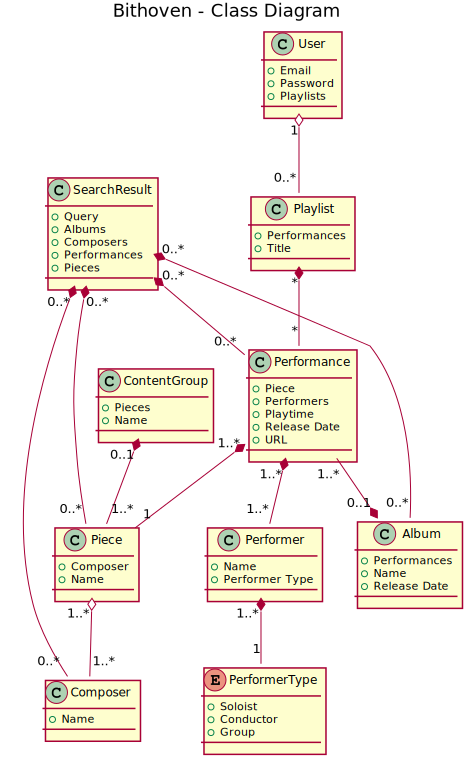
\includegraphics[scale=0.5]{uml.png}

\subsection{Requirements}
\label{project-description-req}

\begin{enumerate}
    \item User can sign up for an account with an e-mail account and password.
    \item User can delete their account when signed in.
    \item User can sign into their account by providing corresponding e-mail
        account and password.
    \item System will provide the user's playlists when signed in.
    \item User can create new playlists.
    \item User can delete playlists.
    \item User can modify name of playlists.
    \item User can add performances to playlists.
    \item User can delete performances from playlists.
    \item User can reorder performances in playlists.
    \item User can search for available performances by providing metadata in a
        free-form search query.
    \item System provides search results from a query grouped into pieces/
        composers/performers/albums.
    \item System can provide metadata for user to explore.
    \item System can list all pieces by composer.
    \item System can list all performances by performer/album.
    \item A piece contains the following metadata: at least 1 composer.
    \item A performance contains the following metadata: 1 piece,
        at least 1 performer, 0 or 1 album.
    \item A performer must have at least one of the following roles in a
        performance: soloist, group, conductor.
    \item A piece may specify a content group.
    \item A piece must have a title.
    \item A performer must have a name. 
    \item An album must have a title.
    \item A composer must have a name.
    \item A performance in an album must specify its track number.
        % FIXME: make better
    \item A performance must contain release date.
    \item An album must contain release date.
    \item A performance must contain its playtime.
    \item A performance must contain a URL to a corresponding song file.
\end{enumerate}
